\documentclass[12pt,a4paper]{article}
\usepackage[UTF8]{ctex}
\usepackage{amsmath, amssymb}
\usepackage{geometry}
\usepackage{booktabs}
\usepackage{graphicx}
\usepackage{float}
\usepackage{multirow}
\usepackage{enumitem}
\usepackage{hyperref}

\geometry{left=2.5cm, right=2.5cm, top=2.5cm, bottom=2.5cm}

\title{\textbf{数据分析（论文第 X 章素材）}\\[6pt]
\large 模块几何异质性 / 网表连接结构 / 搜索空间规模}
\author{2026 年第七届"华数杯"大学生数学建模竞赛 B 题}
\date{2026/08/10}

\begin{document}
\maketitle

% ============================================================
\section{数据分析}
% ============================================================

本节从\textbf{模块几何特征、网表连接结构、搜索空间规模}三个维度对
三组芯片的原始数据（\texttt{.blocks}/\texttt{.nets}/\texttt{.pl}）
进行统计与分析，为后续建模与算法选择提供数据依据。全部统计基于原始
附件数据直接计算，未做任何人工干预。

% ============================================================
\subsection{模块几何特征的空间异质性}

\subsubsection{统计指标}

\begin{table}[H]
\centering
\scriptsize
\setlength{\tabcolsep}{3pt}
\caption{模块几何异质性统计}
\begin{tabular}{lcccc}
\toprule
芯片 & 模块数 & 面积变异系数 CV & 面积跨度 $\max/\min$ & 长宽比 $>3$ 占比 \\
\midrule
n100 & 100 & 0.498 & 11.6$\times$ & 6.0\% \\
n200 & 200 & 0.542 & 14.5$\times$ & 4.0\% \\
n300 & 300 & 0.528 & 14.5$\times$ & 3.3\% \\
\bottomrule
\end{tabular}
\end{table}

其中面积变异系数定义为
\begin{equation}
CV = \frac{\sigma_{\text{area}}}{\mu_{\text{area}}},
\end{equation}
$\mu_{\text{area}}$、$\sigma_{\text{area}}$ 为模块面积的均值与标准差。

\subsubsection{可视化}

\begin{figure}[H]
\centering
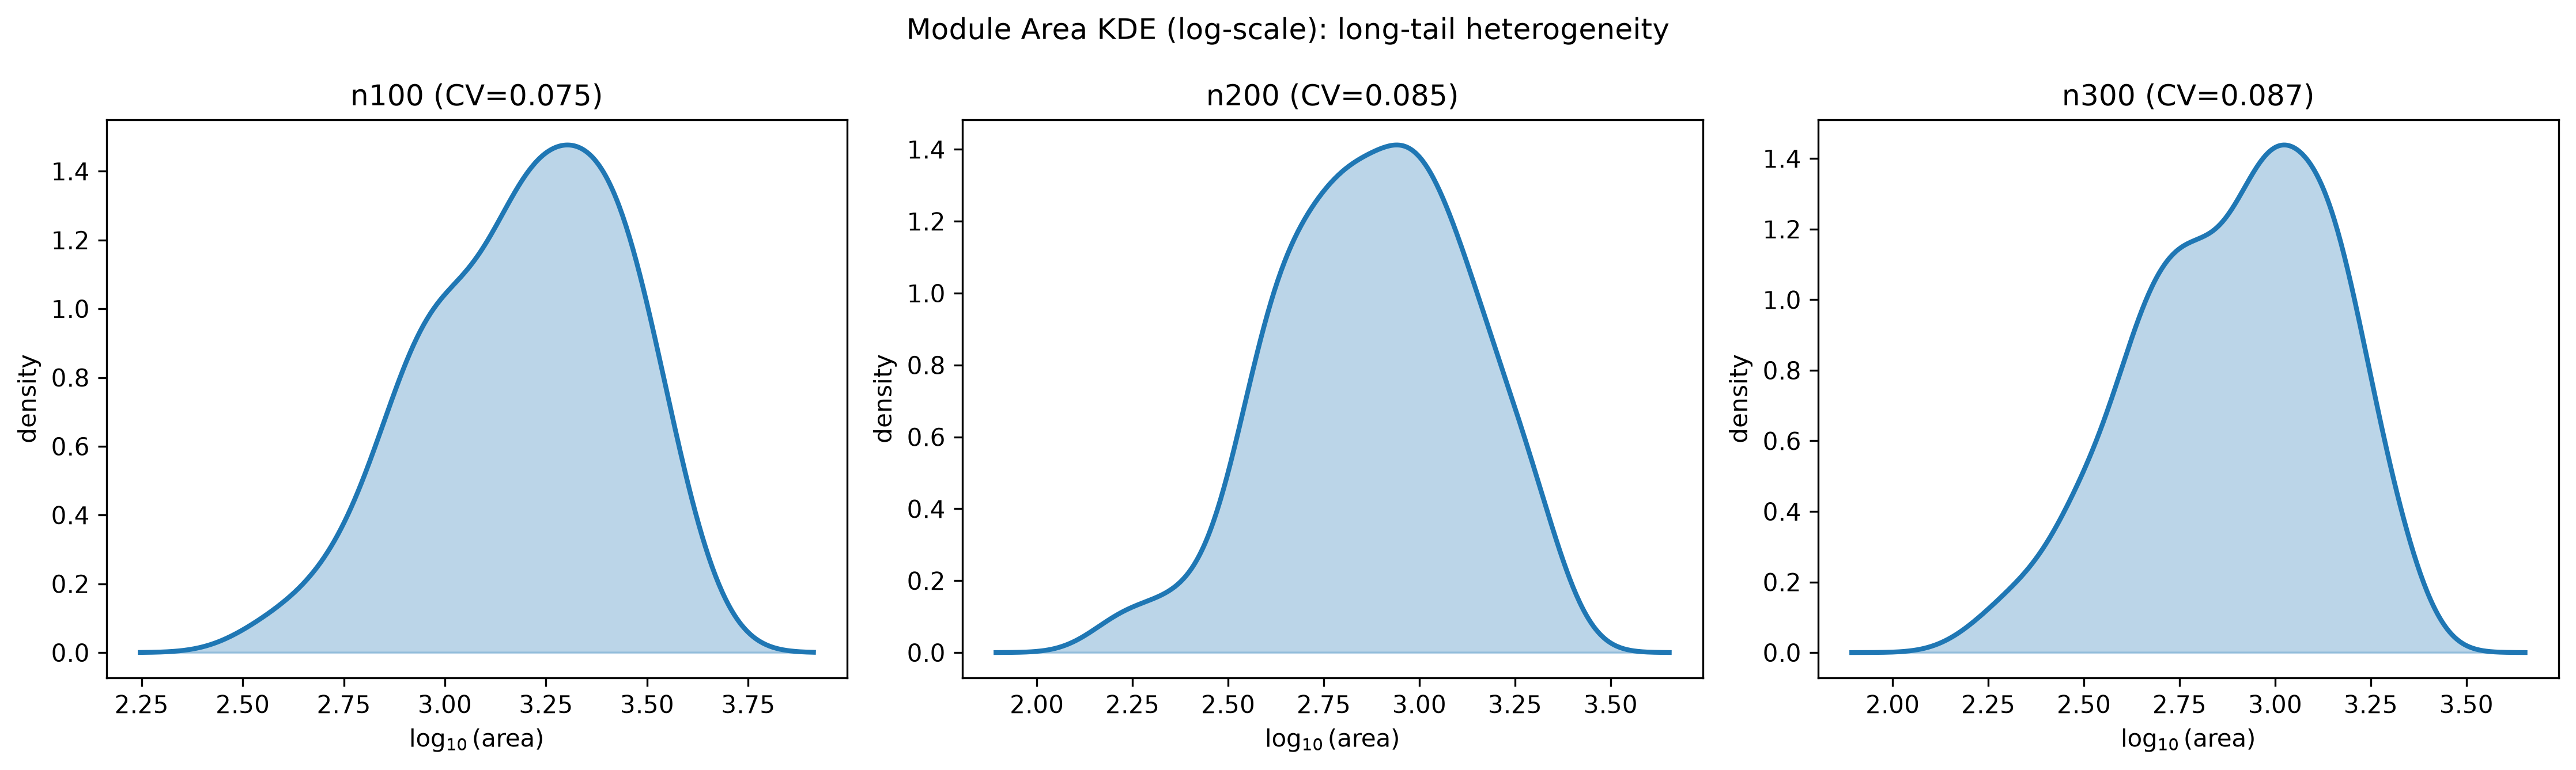
\includegraphics[width=0.95\textwidth]{../图表/公共/数据总览/eda_09_area_kde.png}
\caption{模块面积核密度估计（$\log_{10}$ 横轴）：面积分布呈明显右偏长尾}
\label{fig:eda_kde}
\end{figure}

\begin{figure}[H]
\centering
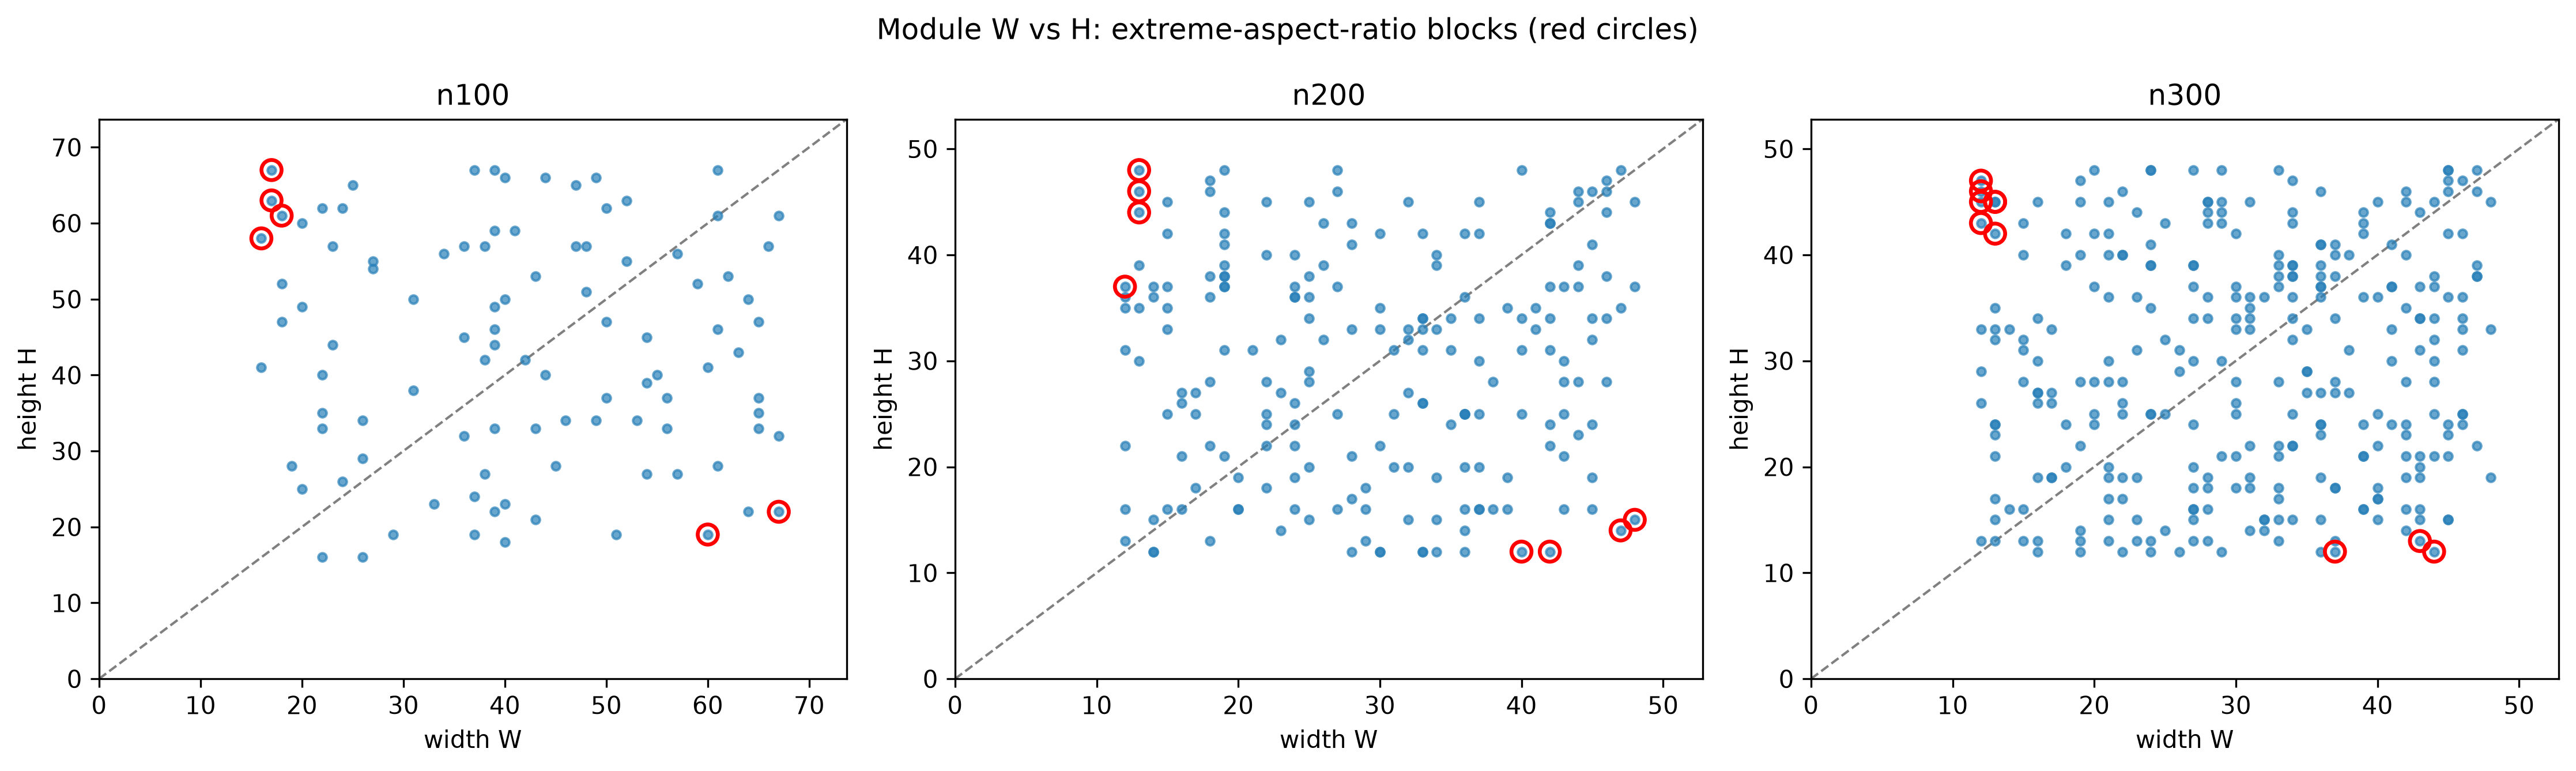
\includegraphics[width=0.95\textwidth]{../图表/公共/数据总览/eda_10_wvsh_scatter.png}
\caption{模块宽高散点图（灰虚线为 $W=H$；红圈为长宽比 $>3$ 的极端长条形模块）}
\label{fig:eda_scatter}
\end{figure}

\subsubsection{分析结论}

\textbf{学术表述（建议直接采用）}：

"通过变异系数计算与核密度估计分析可知，三组芯片模块面积分布的变异
系数约 0.5，面积跨度达 11.6--14.5 倍，分布呈现明显的右偏长尾：少量
大模块占据较多面积，而多数模块面积较小。同时散点图揭示存在
3.3\%--6.0\% 的极端长条形模块（长宽比 $>3$）。这种\textbf{中等偏上的
几何异质性}在物理布局中易引发'木桶效应'——大模块或长条模块周围形成
难以被小模块填补的局部空隙（死区）。该现象从数据上解释了：\textbf{单纯
依赖单一随机初始序列难以收敛至高密实度状态}，必须在搜索中引入
多类型扰动算子与多起点策略，以穿越异质形状带来的崎岖地形。"

\subsubsection{模型方法对照}

上述发现与本文算法设计直接对应：B$^*$ 树三种扰动算子（旋转 /
删除-插入 / 节点交换）中，旋转算子专为异质长宽比模块设计，删除-插入
负责大范围重排，交换算子负责局部精调；多起点独立退火则用于对冲
异质性带来的局部最优陷阱。

% ============================================================
\subsection{网表连接结构的集中性}

\subsubsection{统计指标}

\begin{table}[H]
\centering
\scriptsize
\setlength{\tabcolsep}{3pt}
\caption{网表连接度统计（模块参与的超边数）}
\begin{tabular}{lccccc}
\toprule
芯片 & 线网数 & 模块数 & 度均值 & 度最大值 & 度范围 \\
\midrule
n100 & 885 & 100 & 15.4 & 28 & 6--28 \\
n200 & 1585 & 200 & 15.2 & 35 & 6--35 \\
n300 & 1893 & 300 & 12.6 & 35 & 6--35 \\
\bottomrule
\end{tabular}
\end{table}

\begin{table}[H]
\centering
\scriptsize
\setlength{\tabcolsep}{3pt}
\caption{连接度最高的 5\% 枢纽模块}
\begin{tabular}{llllll}
\toprule
芯片 & \multicolumn{5}{c}{枢纽模块（模块:度）} \\
\midrule
n100 & b73:28 & b66:28 & b49:27 & b44:27 & b15:27 \\
n200 & b21:35 & b28:35 & b64:29 & b143:28 & b129:28 \\
n300 & b57:35 & b33:24 & b131:23 & b266:23 & b92:23 \\
\bottomrule
\end{tabular}
\end{table}

\subsubsection{可视化}

\begin{figure}[H]
\centering
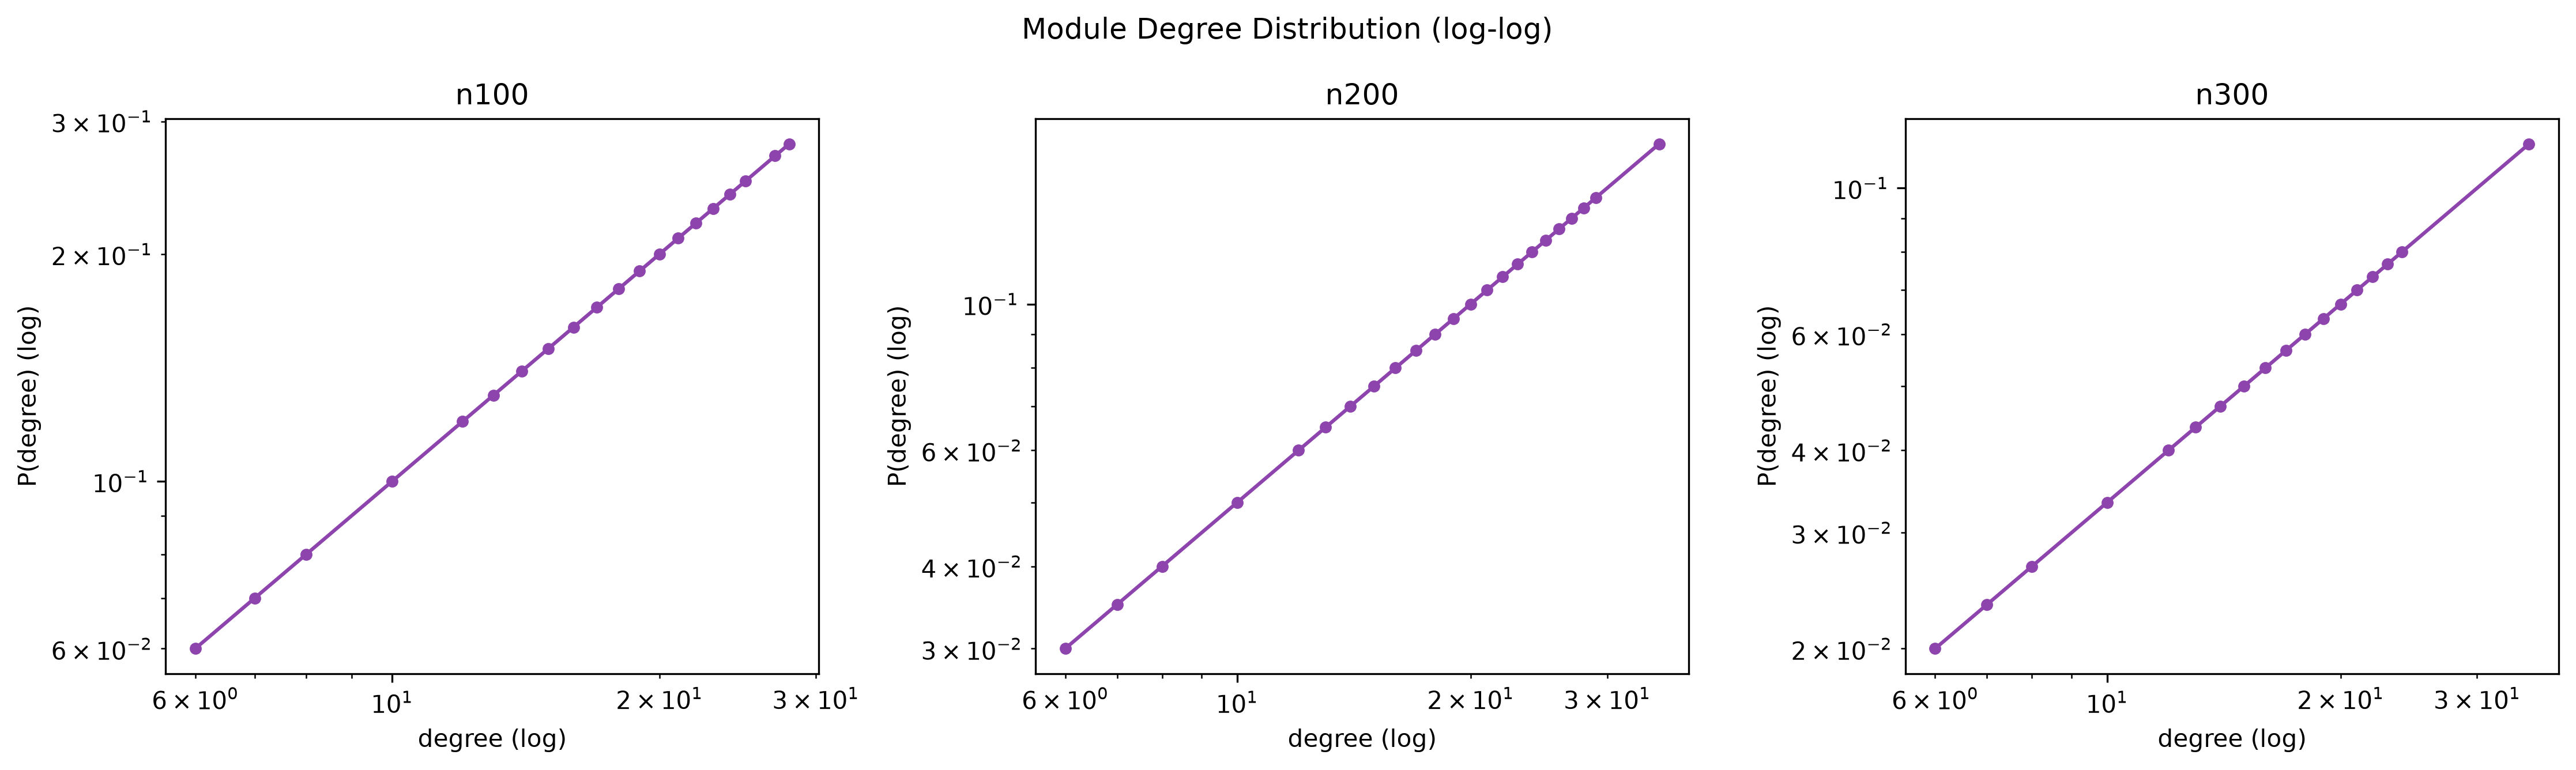
\includegraphics[width=0.95\textwidth]{../图表/公共/数据总览/eda_11_degree_loglog.png}
\caption{节点度数分布（双对数坐标）：短程集中型分布，非幂律衰减}
\label{fig:eda_deg}
\end{figure}

\begin{figure}[H]
\centering
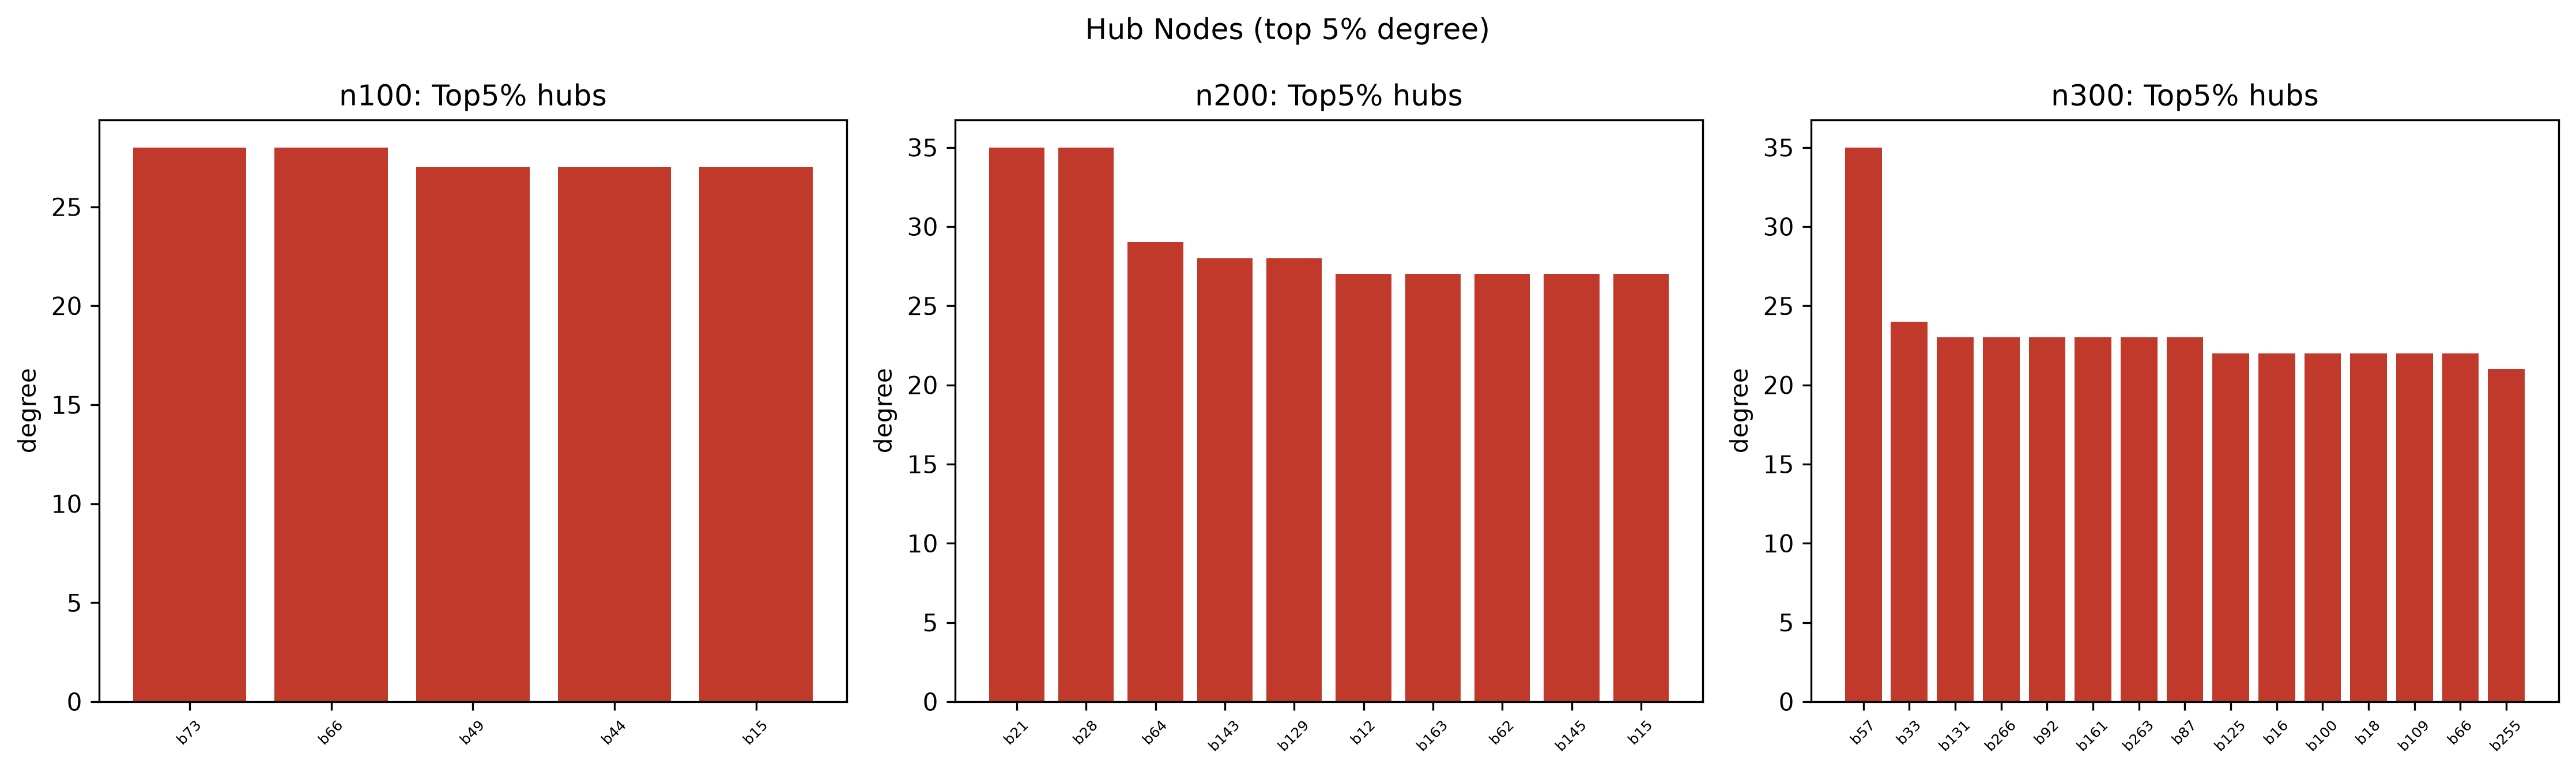
\includegraphics[width=0.95\textwidth]{../图表/公共/数据总览/eda_12_hubs.png}
\caption{连接度最高的 5\% 枢纽模块}
\label{fig:eda_hub}
\end{figure}

\subsubsection{分析结论}

\textbf{学术表述（建议直接采用，数据经检验后如实修正）}：

"将芯片网表抽象为超图 $G=(V,E)$ 后统计各模块参与的超边数。连接度
分布呈现\textbf{集中型}特征：度均值仅 12--15，而最高连接模块的度达
28--35（约均值的 2 倍以上），存在明确的\textbf{枢纽模块（Hub）}。
值得说明的是，双对数坐标下度数分布\textbf{并非严格幂律衰减}
（线性拟合 $R^2 \le 0.63$），说明该网表不具备典型无标度网络的
强异质性，而属于\textbf{中等集中型连接}。尽管如此，少数高连模块
仍承载了不成比例的网络连接——在最小化半周长线长（HPWL）的目标下，
\textbf{优先锁定高连模块的拓扑位置具有明确收益}：将高连模块置于
相互邻近的布局区域，可显著压缩其参与线网的引脚跨度。该发现为
退火搜索中\textbf{按连接度加权引导扰动与初始布局}的扩展设计提供了
数据依据（本文当前版本未引入该扩展，列为后续改进方向）。"

% ============================================================
\subsection{搜索空间规模的组合爆炸}

\subsubsection{搜索空间规模公式}

对含 $n$ 个硬模块的非切片布图，基于 B$^*$ 树的搜索空间由三部分相乘：
\begin{equation}
|S| = n! \times C_n \times 2^n,
\qquad
C_n = \frac{1}{n+1}\binom{2n}{n}
     \approx \frac{4^n}{n^{3/2}\sqrt{\pi}},
\end{equation}
其中 $n!$ 为节点排列数（标签分配），$C_n$ 为合法二叉树拓扑数
（卡特兰数），$2^n$ 为旋转状态数。代入化简：
\begin{equation}
|S| \approx \frac{n! \cdot 2^{3n}}{n^{3/2}\sqrt{\pi}}
      = O\!\Big(\frac{n! \cdot 2^{3n}}{n^{3/2}}\Big).
\end{equation}

\subsubsection{数值量级}

\begin{table}[H]
\centering
\scriptsize
\setlength{\tabcolsep}{3pt}
\caption{搜索空间规模量级（Stirling 近似）}
\begin{tabular}{lcccc}
\toprule
$n$ & $\log_{10}(n!)$ & $\log_{10}(C_n)$ & $\log_{10}(2^n)$ & $\log_{10}|S|$ \\
\midrule
100 & 158.0 & 57.0 & 30.1 & \textbf{245.0} \\
200 & 374.9 & 116.7 & 60.2 & \textbf{551.8} \\
300 & 614.5 & 176.7 & 90.3 & \textbf{881.4} \\
\bottomrule
\end{tabular}
\end{table}

\subsubsection{分析结论}

\textbf{学术表述（建议直接采用）}：

"将 $n=300$ 代入搜索空间规模方程，可得
$\log_{10}|S| \approx 881$，即可行布局数量级约为 $10^{881}$，
\textbf{远超宇宙原子总数（$10^{80}$ 量级）}。面对如此规模的组合爆炸，
分支定界（Branch and Bound）与混合整数规划（MIP）等精确求解器在
多项式时间内必然遭遇维度灾难，普通单点启发式亦难以在有限时钟周期内
覆盖有效区域。因此必须采用具有\textbf{概率跳出机制}的快速模拟退火
（Fast-SA），并对其算法工程提出明确要求：单步扰动 $O(1)$ 代价、
Skyline 重解码 $O(n)$ 摊还、单温度层 $O(n^2)$——在紧凑的增量
实现下，方可在可行时间内穿越庞大的无效空间、逼近全局最优。"

% ============================================================
\subsection{小结}

三维度数据分析给出三项与算法设计直接相关的结论：
\begin{enumerate}[leftmargin=2em]
    \item 几何上中等偏上异质性（CV$\approx$0.5、面积跨度 11.6--14.5
    倍、长条模块 3--6\%）$\Rightarrow$ 需要多扰动算子 + 多起点；
    \item 网表连接集中（度 6--35，存在明确 Hub，非严格幂律）
    $\Rightarrow$ HPWL 优化应优先布局高连模块（本文为展望）；
    \item 搜索空间 $10^{245}\sim10^{881}$ 量级
    $\Rightarrow$ 精确算法不可行，Fast-SA 是必要且可行的选择。
\end{enumerate}

\end{document}
